\graphicspath{{images/}}

\section{\thesection~Introduction}
\label{sec:introduction}

% Expand motivation, describe QFA, discuss alternative approaches.

% Dummy \citet{Lawless2010} citations \citep{Heydari2016} \citep{Addinall2008}.


% Could introduce model organisms first
The bacteria \textit{Eschericia Coli} and yeast \textit{Saccharomyces
  cerevisae} are single-celled microbial organims studied as a model
prokaryote and eukaryote respectively. In favourable conditions,
microbial organisms (such as these) divide exponentially and form
large colonies comprising many individual cells. Cells may be clones
originating from a single cell or (more often in nature) belong to
different genetic strains originating from different individual
cells. For a strain to be successful and dominate a population, it
must (use nutrients efficiently and) divide faster than other strains
in the colony. This has led to the evolution of rapid cell division
and compact genomes in these organisms. \textit{E. Coli} and
\textit{S.  cerevisae} are useful as model organisms because many of
the genes in their compacted genomes have improtant functions which
have been conserved over billions of years of evolution and have
anologues in other species. The eukaryote \textit{S. cerevisae}, is
particularly useful for the study of other eukaryotes such as humans.



% In favourable conditions, microbial organisms such as bacteria and
% yeast divide exponentially and form large colonies comprising many
% individual cells. Cells may be clones originating from a single cell
% or belong to different genetic strains originating from different
% individual cells. For a strain to dominate a population, it must (use
% nutrients efficiently and) divide faster than other strains in the
% colony. This has led to the evolution of rapid cell division and
% compact genomes in such organisms. Many genes have been conserved over
% billions of years of evolution and have anologues in other
% species. The model organism \textit{Saccharomyces cerevisae}, is a
% single-celled eukaryote with a compact genome and is particularly
% useful for the study of other eukaryotes such as humans.
x

the bacteria \textit{Eschericia Coli} and yeast \textit{Saccharomyces cerevisae}p

% Where do cells grow surfaces films.

\subsection{\thesubsection~Subsection}

\begin{Figure}
  \centering
  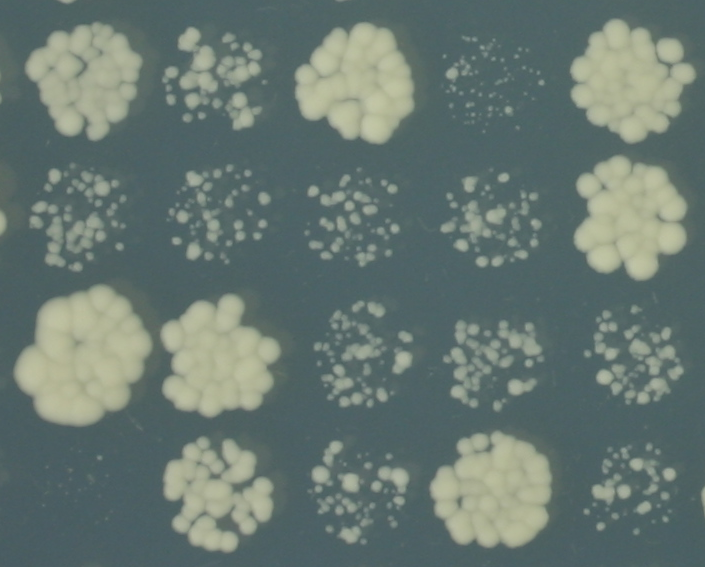
\includegraphics[width=\linewidth]{p15_section/p15_section}
  \captionof{figure}{\textbf{4x5 section of a QFA plate.} Taken from a
    16x24 format solid agar plate inoculated with dilute
    \textit{S. cerevisae} cultures.
  Image captured at \(\sim\)2.5d after inoculation and incubation at
  27\(^{\circ}C\).}
  \label{fig:p15_section}
\end{Figure}


\begin{Figure}
  \centering
  \includegraphics[width=\linewidth]{stripes/final/striped}
  \includegraphics[width=\linewidth]{stripes/final/filled}
  \captionof{figure}{\textbf{An experiment designed to examine
      competition.}\\
    A) QFA plate inocluated with a more concentrated
    \textit{S. Cerevisae} inoculum (no cells inocluated on alternative
    columns).\\
    B) Same as in A, but with strains of similar growth rate
    inoculated in the positions missing in A.}
  \label{fig:stripes_images}
\end{Figure}



%%% Local Variables:
%%% mode: latex
%%% TeX-master: "report"
%%% End:
